\documentclass{article}
\usepackage{graphicx}
\usepackage{amsmath}
\usepackage{amssymb}
\usepackage{listings}
\usepackage[margin=1in]{geometry}
\usepackage{xcolor}
\usepackage{tikz}
\usetikzlibrary{shapes, arrows, positioning, calc}
\usepackage{tcolorbox}
% Define colors for syntax highlighting
\definecolor{codegreen}{rgb}{0,0.6,0}
\definecolor{codegray}{rgb}{0.5,0.5,0.5}
\definecolor{codepurple}{rgb}{0.58,0,0.82}
\definecolor{backcolour}{rgb}{0.95,0.95,0.92}

% Python style for highlighting
\lstdefinestyle{pythonstyle}{
    backgroundcolor=\color{backcolour},   
    commentstyle=\color{codegreen},
    keywordstyle=\color{magenta},
    numberstyle=\tiny\color{codegray},
    stringstyle=\color{codepurple},
    basicstyle=\ttfamily\footnotesize,
    breakatwhitespace=false,         
    breaklines=true,                 
    captionpos=b,                    
    keepspaces=true,                 
    numbers=left,                    
    numbersep=5pt,                  
    showspaces=false,                
    showstringspaces=false,
    showtabs=false,                  
    tabsize=2
}
\lstset{style=pythonstyle}

\title{From Regression to Classification - Loss Functions and Optimization}
\author{Deep Learning Class}
\date{\today}

\begin{document}
\maketitle

\section{From Regression to Classification}

\subsection{Recap: Regression and MSE Loss}

In our previous lectures, we covered linear regression where we predicted continuous values. The mean squared error (MSE) loss function served us well:

$$\mathcal{L}_{\text{MSE}} = \frac{1}{2n} \sum_{i=1}^n (\hat{y}_i - y_i)^2$$

This loss function has nice properties:
\begin{itemize}
\item Convex (single global minimum)
\item Differentiable everywhere
\item Simple gradient: $\nabla_{\hat{y}} \mathcal{L} = \hat{y} - y$
\end{itemize}

\begin{tcolorbox}[colback=yellow!5!white, colframe=orange!50!black, title=Key Question]
Can we use MSE for classification? What happens if we try?
\end{tcolorbox}

\subsection{The Classification Challenge}

Classification differs fundamentally from regression:
\begin{itemize}
\item \textbf{Regression}: Predict continuous values (e.g., house prices)
\item \textbf{Classification}: Predict discrete categories (e.g., cat vs. dog)
\end{itemize}

For classification, we need:
\begin{enumerate}
\item A way to convert raw model outputs (logits) to probabilities
\item A loss function that measures ``how wrong'' our probability predictions are
\end{enumerate}

\section{Binary Classification: The Foundation}

\subsection{From Logits to Probabilities}

Our model produces a raw score (logit) $o \in \mathbb{R}$. We need a probability $p \in [0,1]$.

\textbf{The Sigmoid Function:}
$$\sigma(o) = \frac{1}{1 + e^{-o}} = \frac{e^o}{e^o + 1}$$

\begin{center}
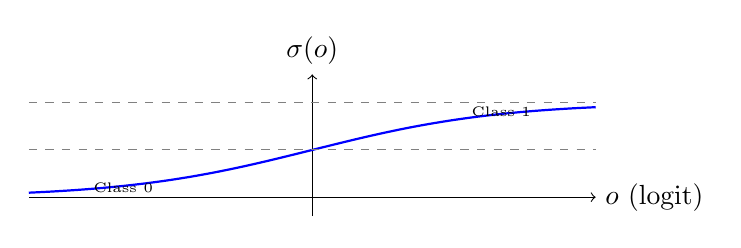
\begin{tikzpicture}[scale=1.2]
\draw[->] (-3,0) -- (3,0) node[right] {$o$ (logit)};
\draw[->] (0,-0.2) -- (0,1.3) node[above] {$\sigma(o)$};
\draw[domain=-3:3, smooth, variable=\x, blue, thick] plot ({\x}, {1/(1+exp(-\x))});
\draw[dashed, gray] (-3, 1) -- (3, 1);
\draw[dashed, gray] (-3, 0.5) -- (3, 0.5);
\node at (-2, 0.1) {{\tiny Class 0}};
\node at (2, 0.9) {{\tiny Class 1}};
\end{tikzpicture}
\end{center}

Properties:
\begin{itemize}
\item Maps $(-\infty, +\infty) \rightarrow (0, 1)$
\item Centered at 0.5 when $o = 0$
\item Smooth and differentiable
\end{itemize}

\subsection{Binary Cross-Entropy Loss}

Given true label $y \in \{0, 1\}$ and predicted probability $\hat{p}$:

$$\mathcal{L}_{\text{BCE}} = -[y \log \hat{p} + (1-y) \log(1-\hat{p})]$$

\begin{tcolorbox}[colback=blue!5!white, colframe=blue!50!black, title=Why Cross-Entropy?]
Cross-entropy measures the ``surprise'' when observing the true outcome given our predicted probabilities. It comes from maximum likelihood estimation:
$$\text{Maximize } P(y|x) = \prod_i p_i^{y_i}(1-p_i)^{1-y_i}$$
Taking negative log gives us cross-entropy loss!
\end{tcolorbox}

\subsection{The Beautiful Gradient}

When we combine sigmoid and cross-entropy, something magical happens:

$$\frac{\partial \mathcal{L}}{\partial o} = \hat{p} - y$$

This is the same form as MSE gradient! The error directly drives the update.

\section{Multi-Class Classification: Softmax and Cross-Entropy}

\subsection{The Softmax Function}

For $K$ classes, we have $K$ logits: $\mathbf{o} = [o_1, ..., o_K]$

\textbf{Softmax} converts these to probabilities:
$$\hat{y}_j = \frac{e^{o_j}}{\sum_{k=1}^K e^{o_k}}$$

\begin{center}
\includegraphics[width=0.6\textwidth]{Module 1/Fig4.1.png}
\\{\tiny Figure from Prince ``Understanding Deep Learning'', Chapter 4}
\end{center}

Key properties:
\begin{itemize}
\item All outputs positive: $\hat{y}_j > 0$
\item Outputs sum to one: $\sum_j \hat{y}_j = 1$
\item Larger logits $\rightarrow$ higher probabilities
\item Invariant to constant shifts: $\text{softmax}(\mathbf{o} + c) = \text{softmax}(\mathbf{o})$
\end{itemize}

\subsection{Cross-Entropy for Multi-Class}

For one-hot encoded true labels $\mathbf{y}$ and predictions $\hat{\mathbf{y}}$:

$$\mathcal{L}_{\text{CE}} = -\sum_{j=1}^K y_j \log \hat{y}_j$$

Since only one $y_j = 1$ (the true class), this simplifies to:
$$\mathcal{L}_{\text{CE}} = -\log \hat{y}_{\text{true class}}$$

\subsection{Information Theory Perspective}

\textbf{Entropy} measures uncertainty in a distribution:
$$H[P] = -\sum_j p_j \log p_j$$

\textbf{Cross-entropy} measures the ``coding cost'' when using distribution $Q$ to encode data from distribution $P$:
$$H(P, Q) = -\sum_j p_j \log q_j$$

\begin{tcolorbox}[colback=green!5!white, colframe=green!50!black, title=Connection to Machine Learning]
Minimizing cross-entropy = Maximizing likelihood = Minimizing KL divergence between predicted and true distributions
\end{tcolorbox}

\subsection{Numerical Stability}

\textbf{Problem:} Computing $e^{o_j}$ can overflow for large logits!

\textbf{Solution:} Use the log-sum-exp trick:
$$\log \sum_j e^{o_j} = \max_k o_k + \log \sum_j e^{o_j - \max_k o_k}$$

\begin{lstlisting}[language=Python, caption=Stable softmax implementation]
def stable_softmax(logits):
    # Subtract max for numerical stability
    max_logits = logits.max(dim=-1, keepdim=True).values
    exp_logits = torch.exp(logits - max_logits)
    return exp_logits / exp_logits.sum(dim=-1, keepdim=True)
\end{lstlisting}

\section{The Gradient Again}

Just as with binary classification, the gradient of softmax + cross-entropy simplifies beautifully:

$$\frac{\partial \mathcal{L}}{\partial o_j} = \hat{y}_j - y_j$$

This is not a coincidence! It emerges from the exponential family of distributions.

\begin{center}
\includegraphics[width=0.7\textwidth]{Module 1/Fig4.2.png}
\\{\tiny Figure from Prince ``Understanding Deep Learning'', Chapter 4}
\end{center}

\section{Fitting Models: Stochastic Gradient Descent}

\subsection{From Full Batch to Stochastic Updates}

Three variants of gradient descent:

\begin{enumerate}
\item \textbf{Batch Gradient Descent:}
$$\mathbf{w}_{t+1} = \mathbf{w}_t - \eta \nabla_\mathbf{w} \mathcal{L}(\mathbf{w}_t) = \mathbf{w}_t - \eta \frac{1}{n} \sum_{i=1}^n \nabla_\mathbf{w} \ell_i(\mathbf{w}_t)$$
\begin{itemize}
\item Uses entire dataset
\item Exact gradient
\item Slow per iteration
\end{itemize}

\item \textbf{Stochastic Gradient Descent (SGD):}
$$\mathbf{w}_{t+1} = \mathbf{w}_t - \eta \nabla_\mathbf{w} \ell_i(\mathbf{w}_t)$$
\begin{itemize}
\item Uses single sample
\item Noisy gradient
\item Fast per iteration
\end{itemize}

\item \textbf{Minibatch SGD:}
$$\mathbf{w}_{t+1} = \mathbf{w}_t - \eta \frac{1}{|B|} \sum_{i \in B} \nabla_\mathbf{w} \ell_i(\mathbf{w}_t)$$
\begin{itemize}
\item Uses batch $B$ of samples
\item Balanced approach
\item Most commonly used
\end{itemize}
\end{enumerate}

\subsection{Why Minibatches?}

\begin{center}
\includegraphics[width=0.8\textwidth]{Module 1/Fig12.5.png}
\\{\tiny Figure from Prince ``Understanding Deep Learning'', Chapter 12}
\end{center}

\textbf{Computational Efficiency:}
\begin{itemize}
\item Matrix operations are faster than vector operations
\item Better GPU utilization
\item Amortizes memory access overhead
\end{itemize}

\textbf{Statistical Benefits:}
\begin{itemize}
\item Reduces gradient variance by factor of $\sqrt{|B|}$
\item Still maintains stochasticity for escaping local minima
\item Enables certain techniques (e.g., batch normalization)
\end{itemize}

\subsection{Choosing Batch Size}

\begin{center}
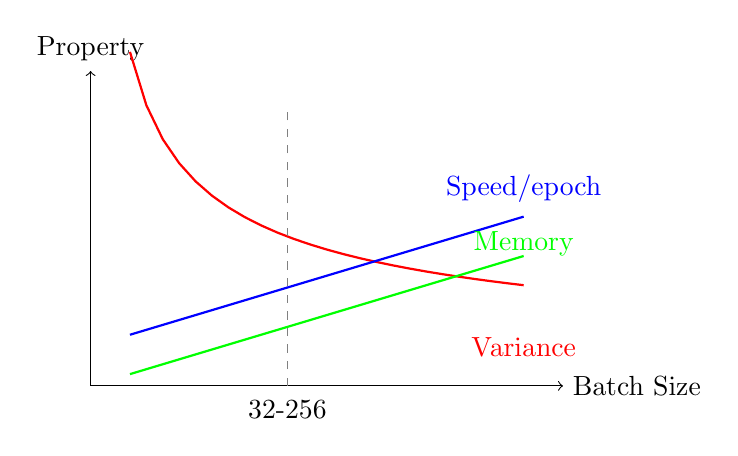
\begin{tikzpicture}[scale=1]
\draw[->] (0,0) -- (6,0) node[right] {Batch Size};
\draw[->] (0,0) -- (0,4) node[above] {Property};

% Gradient variance
\draw[thick, red, domain=0.5:5.5] plot (\x, {3/sqrt(\x)});
\node[red] at (5.5, 0.5) {Variance};

% Computation time
\draw[thick, blue, domain=0.5:5.5] plot (\x, {0.5 + 0.3*\x});
\node[blue] at (5.5, 2.5) {Speed/epoch};

% Memory usage
\draw[thick, green, domain=0.5:5.5] plot (\x, {0.3*\x});
\node[green] at (5.5, 1.8) {Memory};

% Sweet spot
\draw[dashed, gray] (2.5, 0) -- (2.5, 3.5);
\node at (2.5, -0.3) {32-256};
\end{tikzpicture}
\end{center}

Typical batch sizes: 32, 64, 128, 256 (powers of 2 for hardware efficiency)

\section{Initialization Matters!}

\subsection{The Problem with Poor Initialization}

\begin{center}
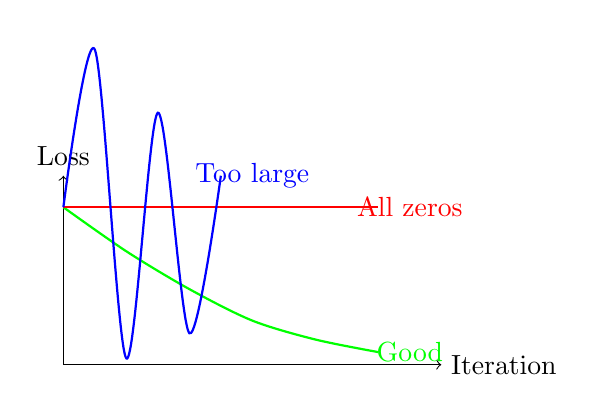
\begin{tikzpicture}[scale=0.8]
\draw[->] (0,0) -- (6,0) node[right] {Iteration};
\draw[->] (0,0) -- (0,3) node[above] {Loss};

% Good initialization
\draw[green, thick] plot[smooth] coordinates {(0,2.5) (1,1.8) (2,1.2) (3,0.7) (4,0.4) (5,0.2)};
\node[green] at (5.5, 0.2) {Good};

% Zero initialization
\draw[red, thick] plot[smooth] coordinates {(0,2.5) (1,2.5) (2,2.5) (3,2.5) (4,2.5) (5,2.5)};
\node[red] at (5.5, 2.5) {All zeros};

% Too large
\draw[blue, thick] plot[smooth] coordinates {(0,2.5) (0.5,5) (1,0.1) (1.5,4) (2,0.5) (2.5,3)};
\node[blue] at (3, 3) {Too large};
\end{tikzpicture}
\end{center}

Problems with bad initialization:
\begin{itemize}
\item \textbf{All zeros:} Symmetry breaking fails, neurons learn same function
\item \textbf{Too small:} Vanishing gradients, slow learning
\item \textbf{Too large:} Exploding gradients, unstable training
\end{itemize}

\subsection{Initialization Strategies}

\textbf{1. Xavier/Glorot Initialization (for sigmoid/tanh):}
$$\mathbf{W} \sim \mathcal{N}\left(0, \sqrt{\frac{2}{n_{\text{in}} + n_{\text{out}}}}\right)$$

\textbf{2. He Initialization (for ReLU):}
$$\mathbf{W} \sim \mathcal{N}\left(0, \sqrt{\frac{2}{n_{\text{in}}}}\right)$$

\textbf{Principle:} Maintain variance of activations and gradients across layers.

\begin{lstlisting}[language=Python, caption=Initialization in practice]
# PyTorch example
def init_weights(m):
    if isinstance(m, nn.Linear):
        # He initialization for ReLU
        nn.init.kaiming_normal_(m.weight, mode='fan_in', 
                                nonlinearity='relu')
        # Zero bias
        nn.init.zeros_(m.bias)

model.apply(init_weights)
\end{lstlisting}

\section{Epochs and Training Dynamics}

\subsection{What is an Epoch?}

\begin{tcolorbox}[colback=yellow!5!white, colframe=yellow!50!black, title=Definition]
One \textbf{epoch} = One complete pass through the entire training dataset
\end{tcolorbox}

With minibatch SGD:
\begin{itemize}
\item Dataset size: $n$ samples
\item Batch size: $B$ samples
\item Steps per epoch: $\lceil n/B \rceil$
\end{itemize}

\subsection{Training Over Multiple Epochs}

\begin{center}
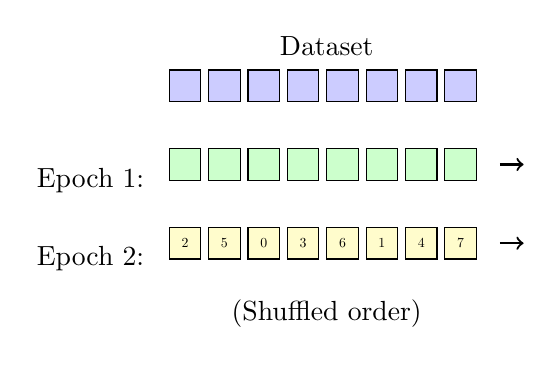
\begin{tikzpicture}[scale=1]
% Dataset
\foreach \i in {0,...,7} {
    \draw[fill=blue!20] ({\i*0.5}, 3) rectangle ({\i*0.5+0.4}, 3.4);
}
\node at (2, 3.7) {Dataset};

% Epoch 1
\node at (-1, 2) {Epoch 1:};
\foreach \i in {0,...,7} {
    \draw[fill=green!20] ({\i*0.5}, 2) rectangle ({\i*0.5+0.4}, 2.4);
}
\draw[->, thick] (4.2, 2.2) -- (4.5, 2.2);

% Epoch 2
\node at (-1, 1) {Epoch 2:};
\foreach \i in {0,...,7} {
    \pgfmathparse{int(mod(\i*3+2, 8))}
    \edef\j{\pgfmathresult}
    \draw[fill=yellow!20] ({\i*0.5}, 1) rectangle ({\i*0.5+0.4}, 1.4);
    \node[scale=0.5] at ({\i*0.5+0.2}, 1.2) {\j};
}
\draw[->, thick] (4.2, 1.2) -- (4.5, 1.2);

\node at (2, 0.3) {(Shuffled order)};
\end{tikzpicture}
\end{center}

Key points:
\begin{itemize}
\item Each epoch sees all data exactly once
\item Data is shuffled between epochs (important!)
\item Multiple epochs allow learning complex patterns
\end{itemize}

\subsection{Learning Dynamics Across Epochs}

\begin{center}
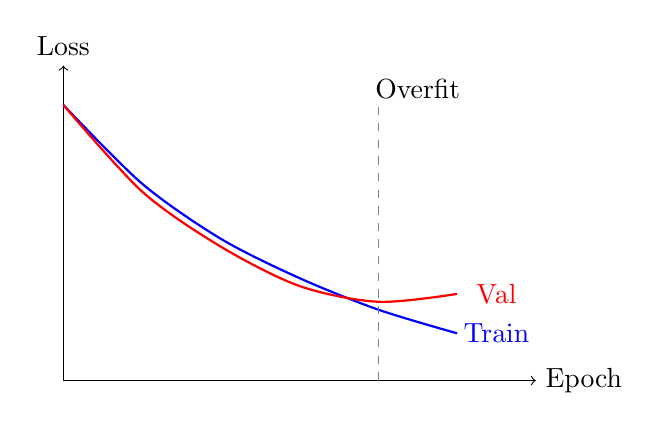
\begin{tikzpicture}[scale=1]
\draw[->] (0,0) -- (6,0) node[right] {Epoch};
\draw[->] (0,0) -- (0,4) node[above] {Loss};

% Training loss
\draw[thick, blue] plot[smooth] coordinates 
    {(0,3.5) (1,2.5) (2,1.8) (3,1.3) (4,0.9) (5,0.6)};
\node[blue] at (5.5, 0.6) {Train};

% Validation loss
\draw[thick, red] plot[smooth] coordinates 
    {(0,3.5) (1,2.4) (2,1.7) (3,1.2) (4,1.0) (5,1.1)};
\node[red] at (5.5, 1.1) {Val};

% Overfitting region
\draw[dashed, gray] (4, 0) -- (4, 3.5);
\node at (4.5, 3.7) {Overfit};
\end{tikzpicture}
\end{center}

\textbf{Early epochs:}
\begin{itemize}
\item Rapid decrease in loss
\item Learning general patterns
\item Large weight updates
\end{itemize}

\textbf{Later epochs:}
\begin{itemize}
\item Slower improvement
\item Risk of overfitting
\item May need learning rate decay
\end{itemize}

\section{The Complete SGD Algorithm}

\begin{lstlisting}[language=Python, caption=Minibatch SGD implementation]
def train_model(model, data_loader, num_epochs, learning_rate):
    # Initialize weights (He initialization for ReLU)
    for m in model.modules():
        if isinstance(m, nn.Linear):
            nn.init.kaiming_normal_(m.weight)
            nn.init.zeros_(m.bias)
    
    optimizer = torch.optim.SGD(model.parameters(), lr=learning_rate)
    criterion = nn.CrossEntropyLoss()
    
    for epoch in range(num_epochs):
        # Shuffle data each epoch (handled by DataLoader)
        epoch_loss = 0.0
        
        for batch_idx, (X_batch, y_batch) in enumerate(data_loader):
            # Forward pass
            logits = model(X_batch)
            loss = criterion(logits, y_batch)
            
            # Backward pass
            optimizer.zero_grad()  # Clear previous gradients
            loss.backward()        # Compute gradients
            optimizer.step()       # Update weights: w = w - lr * grad
            
            epoch_loss += loss.item()
        
        # Print epoch statistics
        avg_loss = epoch_loss / len(data_loader)
        print(f'Epoch {epoch+1}/{num_epochs}, Loss: {avg_loss:.4f}')
    
    return model
\end{lstlisting}

\subsection{Key Components}

\begin{enumerate}
\item \textbf{Initialization:} Start with appropriate random weights
\item \textbf{Shuffle:} Randomize data order each epoch
\item \textbf{Minibatch:} Process $B$ samples at a time
\item \textbf{Gradient step:} $\mathbf{w} \leftarrow \mathbf{w} - \eta \nabla \mathcal{L}$
\item \textbf{Repeat:} Multiple epochs until convergence
\end{enumerate}

\section{Practical Considerations}

\subsection{Learning Rate Selection}

\begin{center}
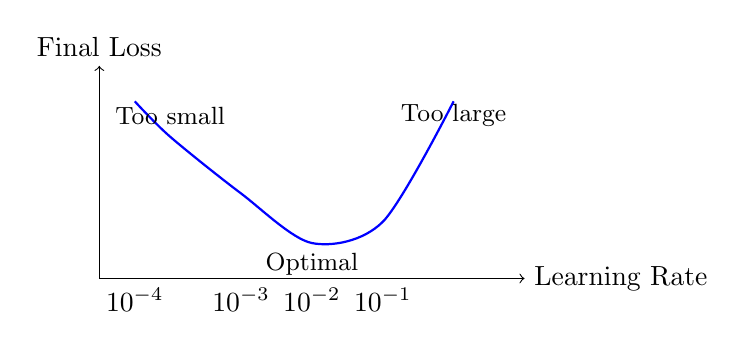
\begin{tikzpicture}[scale=0.9]
\draw[->] (0,0) -- (6,0) node[right] {Learning Rate};
\draw[->] (0,0) -- (0,3) node[above] {Final Loss};

% Loss curve
\draw[thick, blue] plot[smooth] coordinates 
    {(0.5,2.5) (1,2) (2,1.2) (3,0.5) (4,0.8) (5,2.5)};

\node at (0.5, -0.3) {$10^{-4}$};
\node at (2, -0.3) {$10^{-3}$};
\node at (3, -0.3) {$10^{-2}$};
\node at (4, -0.3) {$10^{-1}$};

\node at (1, 2.3) {\small Too small};
\node at (3, 0.2) {\small Optimal};
\node at (5, 2.3) {\small Too large};
\end{tikzpicture}
\end{center}

\textbf{Learning rate schedules:}
\begin{itemize}
\item Constant: $\eta_t = \eta_0$
\item Step decay: $\eta_t = \eta_0 \cdot \gamma^{\lfloor t/s \rfloor}$
\item Exponential: $\eta_t = \eta_0 \cdot \gamma^t$
\item Cosine annealing: $\eta_t = \eta_{min} + \frac{1}{2}(\eta_{max} - \eta_{min})(1 + \cos(\frac{t\pi}{T}))$
\end{itemize}

\subsection{Batch Size Trade-offs}

\begin{center}
\begin{tabular}{|l|c|c|c|}
\hline
\textbf{Batch Size} & \textbf{1} & \textbf{32-256} & \textbf{Full} \\
\hline
Gradient Noise & High & Moderate & None \\
Memory Usage & Low & Moderate & High \\
Computation/epoch & Slow & Fast & Fast \\
Generalization & Good & Good & Poor \\
Escape Local Minima & Easy & Moderate & Hard \\
\hline
\end{tabular}
\end{center}

\subsection{Monitoring Training}

Key metrics to track:
\begin{itemize}
\item Training loss (should decrease)
\item Validation loss (watch for overfitting)
\item Gradient norms (check for vanishing/exploding)
\item Learning rate (if using schedule)
\item Accuracy/other metrics
\end{itemize}

\section{Summary}

\begin{tcolorbox}[colback=blue!5!white, colframe=blue!50!black, title=Key Takeaways]
\begin{enumerate}
\item \textbf{Loss Functions:}
    \begin{itemize}
    \item MSE for regression
    \item Cross-entropy for classification
    \item Both give gradient $\propto$ (prediction - target)
    \end{itemize}
    
\item \textbf{Softmax + Cross-Entropy:}
    \begin{itemize}
    \item Natural pairing from maximum likelihood
    \item Numerically stable implementation crucial
    \item Simple, interpretable gradients
    \end{itemize}
    
\item \textbf{SGD Optimization:}
    \begin{itemize}
    \item Minibatches balance efficiency and stochasticity
    \item Typical batch sizes: 32-256
    \item Shuffle data between epochs
    \end{itemize}
    
\item \textbf{Initialization:}
    \begin{itemize}
    \item Critical for convergence
    \item Xavier for sigmoid/tanh
    \item He for ReLU
    \end{itemize}
    
\item \textbf{Training Process:}
    \begin{itemize}
    \item Multiple epochs to learn patterns
    \item Monitor for overfitting
    \item Adjust learning rate as needed
    \end{itemize}
\end{enumerate}
\end{tcolorbox}

\section{Looking Ahead}

Next lecture, we'll cover:
\begin{itemize}
\item Backpropagation: How gradients are computed efficiently
\item Advanced optimizers: Momentum, Adam, and beyond
\item Regularization techniques
\item Practical training tricks
\end{itemize}

\section{Practical Exercise}

Implement a complete training pipeline for multi-class classification:

\begin{lstlisting}[language=Python, caption=Exercise template]
import torch
import torch.nn as nn
from torch.utils.data import DataLoader, TensorDataset

# 1. Generate synthetic 3-class dataset
torch.manual_seed(42)
n_samples = 1000
n_features = 20
n_classes = 3

X = torch.randn(n_samples, n_features)
y = torch.randint(0, n_classes, (n_samples,))

# 2. Create data loaders
dataset = TensorDataset(X, y)
train_loader = DataLoader(dataset, batch_size=32, shuffle=True)

# 3. Define model
class Classifier(nn.Module):
    def __init__(self, input_dim, hidden_dim, output_dim):
        super().__init__()
        self.fc1 = nn.Linear(input_dim, hidden_dim)
        self.relu = nn.ReLU()
        self.fc2 = nn.Linear(hidden_dim, output_dim)
    
    def forward(self, x):
        x = self.fc1(x)
        x = self.relu(x)
        x = self.fc2(x)  # Return logits
        return x

# 4. Initialize model with proper initialization
model = Classifier(n_features, 64, n_classes)

# TODO: Add He initialization
# TODO: Train for multiple epochs
# TODO: Track and plot training loss
# TODO: Experiment with different batch sizes
# TODO: Implement learning rate scheduling
\end{lstlisting}

\end{document}